\section{The principles of physics}\index{Measurements}\index{Reference frame}
There is no physics without measurements, otherwise it would be just mathematics.\\
As theoretical physicists there is no need to know the whole procedure behind experiments and measurements, we just need to know that what we are studying can be measured and therefore our assumptions must be verified by some kind of experimental result.\\ Measurements must, from the definition of the scientific method, be reproducible: this means that everybody, everywhere in the universe should be able to replicate the results of a certain experiment. Since the outcome of an experiment is determined by the laws of nature and everybody should agree on such outcome, it seems reasonable to think that laws of nature should be the same for everybody.\\ Actually this isn't so obvious and thus require some further understanding of the reality. In order to proceed we remind the intrinsic experimental nature of physics, in fact we are going to define some \emph{principles}: those are fundamentally different from the axioims of mathematic. The principles of physics are based always on some empirical observation and thus they are not arbitrary.

\subsection{Space and time} \index{Space} \index{Time}
First we are going to assume the existence of space and time: this assumption is actually obvious since we experience every day the space, in which we live in, and the flow of time. It is less obvious which mathematical proprieties to give to those two concepts. We will assume from empirical evidence that:
\begin{itemize}
    \item \textbf{space} is \emph{3 dimensional, isotropic, homogeneous} and it obeys \emph{euclidean geometry};
    \item \textbf{time} is \emph{1 dimensional, isotropic and homogeneous} too. 
\end{itemize}
Given these proprieties space and time can be studied as an affine space (since they are isotropic and homogeneous) that we call \textbf{universe}. 

\marginnote{
    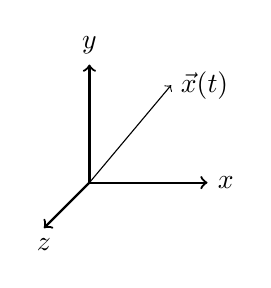
\begin{tikzpicture}
        % Assi cartesiani
        \draw[->,thick] (0,0,0) -- (1.5,0,0) node[right] {$x$};
        \draw[->,thick] (0,0,0) -- (0,1.5,0) node[above] {$y$};
        \draw[->,thick] (0,0,0) -- (0,0,1.5) node[below] {$z$};
        \draw[->] (0,0,0) -- (1.5,1.7,1.2) node[right] {$\vec x(t)$};
    \end{tikzpicture}
    \small The vector $\vec x(t)$ in the $\mathbb{R}^3$ vector space of the reference frame.
}
A body moving in space will result in a curve in the universe. If we want to describe that motion it is convenient to use a set of coordinate in a vector space: this can be done by choosing an arbitrary point in time, from which we will start to measure time itself, and arbitrary point in space, as the null vector, and then three linearly independent vectors as basis. Let's observe that all of these choices are arbitrary only if space and time are isotropic and homogeneous, as we assumed in the beginning.\\ The procedure described is the mathematical equivalent of choosing a \textbf{reference frame}\index{Inertial reference frame} which allow us to describe motion as the curve:
\begin{equation*}
    \vec x(t),\qquad \vec x\in \mathbb{R}^3,\ t\in\mathbb{R}.
\end{equation*}
\subsection{Inertial reference frames and relativity}
Now we have all the tools to discuss the problem, that we mentioned at the beginning of this chapter, of having the same laws of nature for everybody.

First we need to define a special type of reference frame, called \textbf{inertial}. 
\marginnote{
    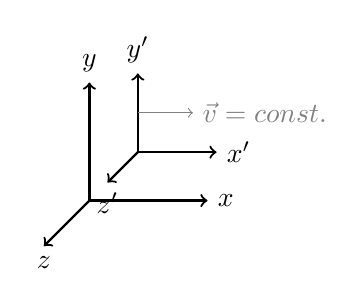
\begin{tikzpicture}
        % Assi cartesiani
        \draw[->,thick] (0,0,0) -- (1.5,0,0) node[right] {$x$};
        \draw[->,thick] (0,0,0) -- (0,1.5,0) node[above] {$y$};
        \draw[->,thick] (0,0,0) -- (0,0,1.5) node[below] {$z$};

        \draw[->,thick] (1,1,1) -- (2,1,1) node[right] {$x'$};
        \draw[->,thick] (1,1,1) -- (1,2,1) node[above] {$y'$};
        \draw[->,thick] (1,1,1) -- (1,1,2) node[below] {$z'$};
        \draw[->,gray] (1,1.5,1) -- (1.7,1.5,1) node[right] {$\vec v=\text{const.}$};
        
    \end{tikzpicture}
    \small The primed reference frame moving with constant velocity $\vec v$ and thus being inertial.
}
\begin{definition}
    An inertial reference frame is such if and only if the motion of its origin, seen in another inertial reference frame, is uniform and rectilinear.
\end{definition}
This definition might seem not well-structured, since we need a preexisting reference frame. Using other principles of physics we will acquire new ways to determine if a reference frame is inertial.

The notion of inertial reference frame is totally useless until we postulate the \textbf{principle of relativity}, as the solution of our initial problem. 
\begin{principle}[of Relativity]
    All the laws of physics are the same in all inertial reference frames.
\end{principle} 
In this way it makes totally sense to describe phenomena and pretend to determine the universal laws of nature from experiments and thus physics can exist only if these principles hold, or some kind of their generalization.\\ 

What we have assumed until now represent the most fundamental axioms of physics: every theory, from classical mechanics, to relativity, up to quantum mechanics, needs these assumptions and by adding others they can be constructed.

\subsection{Transformations of inertial reference frames}

\section{Principle of least action}\index{Principle of least action}\index{Lagrangian}\index{Action}
The most important fundamental principle of physics is, without any doubt, the \textbf{principle of least action}. This principle gives us a way to describe the time evolution of a system: firstly of mechanical systems and then, by its generalization, to fields. 

In order to describe a mechanical system we define a function $L$ called \textbf{lagrangian}, which depends on the \emph{generalized coordinates} of the systems $q_1,q_2,\dots,q_n$ and their time derivatives $\dot q_1,\dot q_2,\dots,\dot q_n$\footnote{$\dot q\triangleq \frac{dq}{dt}$.}.

\begin{principle}[Least action]\label{princ:LeastAction}
    \marginnote{
    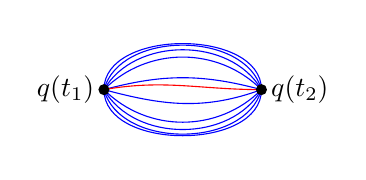
\begin{tikzpicture}
        % Definizione dei punti A e B
        \coordinate (A) at (-1,0);
        \coordinate (B) at (1,0);
        
        % Disegno dei percorsi curvi
        \draw[blue] (A) to[out=45, in=135] (B);
        \draw[blue] (A) to[out=60, in=120] (B);
        \draw[blue] (A) to[out=75, in=105] (B);
        \draw[blue] (A) to[out=90, in=90] (B);
        \draw[blue] (A) to[out=15, in=165] (B);
        \draw[red] (A) to[out=10, in=180] (B);
        \draw[blue] (A) to[out=-15, in=-160] (B);
        \draw[blue] (A) to[out=-90, in=-90] (B);
        \draw[blue] (A) to[out=-45, in=-135] (B);
        \draw[blue] (A) to[out=-60, in=-120] (B);
        \draw[blue] (A) to[out=-75, in=-105] (B);

        % Disegno dei punti A e B
        \fill (A) circle (2pt) node[left] {$q(t_1)$};
        \fill (B) circle (2pt) node[right] {$q(t_2)$};
      \end{tikzpicture}
      \small Different evolutions of a system through time; only the red one minimize the action and thus is the real one. 
}
  The time evolution of a mechanical system, described by $n$ generalized coordinates $q_1,q_2,\dots,q_n$, between $t_1$ and $t_2$, with fixed initial and final coordinates, is given by the functions that minimize the \textbf{action} functional $\mathcal{S}$.
  \begin{equation}
    \delta\mathcal{S} =\delta\int_{t_1}^{t_2}dt\ L(q_1(t),q_2(t),\dots,q_n(t),\dot q_1(t),\dot q_2(t),\dots,\dot q_n(t),t)=0. 
    \label{LeastAction}
  \end{equation}
\end{principle}
In this way we just need to find the right lagrangian to describe the system in the right framework (classical or relativistic) and then the approach to integrate the system will be the same. 
\subsection{Euler-Lagrange equations}
Given the principle \ref{princ:LeastAction} we can derive a set of differential equations which solutions are the equations of motion, this can be done through the \textbf{Euler-Lagrange equations}.
\begin{theorem}
    The functions that make stationary the action functional (defined in \eqref{LeastAction}) are the solutions of the differential equations given by:
    \begin{equation}\label{Euler-Lagrange}
        \frac{d}{dt}\frac{\partial L}{\partial \dot q_i}-\frac{\partial L}{\partial q_i}=0,\qquad \forall i\in\{1,2,\dots,n\}.
    \end{equation}
\end{theorem}
\begin{proof}
    We will use the shorthand for all the generalized coordinates $q=(q_1,q_2,\dots,q_n)$.\\In order to find the set of functions $q(t)$ which make stationary the action we will consider a second arbitrary set of functions $\delta q(t)=(\delta q_1(t),\delta q_2(t),\dots,\delta q_n(t))$ such as these are arbitrary small in the interval $(t_1,t_2)$ and they vanish for $t=t_1$ and $t=t_2$. This last requirement is such that $q(t)+\delta q(t)$ has the same initial and finale coordinates of $q(t)$ in the interval $[t_1,t_2]$.\\ The variation of the action given by $q(t)\rightarrow q(t)+\delta q(t)$ is:
    \begin{equation*}
        \delta \mathcal{S}=\mathcal{S}[q(t)+\delta q(t)]-\mathcal{S}[q(t)]=\int_{t_1}^{t_2}dt\ \bigg[L\big(q(t)+\delta q(t),\dot q(t)+\delta \dot q(t),t\big)-L\big(q(t),\dot q(t),t\big)\bigg].
    \end{equation*}
    Expanding $L\big(q(t)+\delta q(t),\dot q(t)+\delta \dot q(t),t\big)$ in Taylor series the integral becomes (at the first order of expansion):
    \begin{equation*}
        \delta \mathcal{S}\approx\int_{t_1}^{t_2}dt\ \bigg[\frac{\partial L}{\partial q}\delta q+\frac{\partial L}{\partial \dot q}\delta \dot q\bigg]=\int_{t_1}^{t_2}dt\ \sum_{i=0}^{n}\bigg[\frac{\partial L}{\partial q_i}\delta q_i+\frac{\partial L}{\partial \dot q_i}\delta \dot q_i\bigg]
    \end{equation*}
    From integration by parts of the terms containing $\delta \dot q_i=\frac{d}{dt}\delta q_i$ and considering that $\delta q_i(t_1)=\delta q_i(t_2)=0$, we get:
    \begin{equation*}
        \delta \mathcal{S}\approx\bigg[\frac{\partial L}{\partial\dot q_i}\delta q_i\bigg]_{t_1}^{t_2}+\int_{t_1}^{t_2}dt\ \sum_{i=0}^{n}\bigg[\frac{\partial L}{\partial q_i}\delta q_i-\frac{d}{dt}\frac{\partial L}{\partial \dot q_i}\delta q_i\bigg]=\int_{t_1}^{t_2}dt\ \sum_{i=0}^{n}\bigg[\frac{\partial L}{\partial q_i}-\frac{d}{dt}\frac{\partial L}{\partial\dot q_i}\bigg]\delta q_i=0
    \end{equation*}
    In order to have $\delta \mathcal{S}=0$ the integrand must vanish and, considering that $\delta q_i$ is an arbitrary function, all the terms in square brackets should independently go to zero, resulting in \eqref{Euler-Lagrange}.
\end{proof}
Let's observe two consequences of this formulation of the principle of least action:
\begin{itemize}
    \item since in the lagrangian appear only first time derivatives, the differential equations resulting from \eqref{Euler-Lagrange} are second order ordinary differential equations and thus every solution is unique given initial positions and velocities.
    \item if in the lagrangian doesn't appear one coordinate $q_k$ then:
    \begin{equation*}
        \frac{\partial L}{\partial q_k}=0\ \Rightarrow\ \frac{d}{dt}\frac{\partial L}{\partial \dot q_k}=0\ \Rightarrow\ \frac{\partial L}{\partial \dot q_k}=\text{const}.
    \end{equation*}
\end{itemize}
\subsection{Noether's theorem}
\subsection{Euler-Lagrange equations for fields}
As we have already said, the principle of least action (Principle \ref{princ:LeastAction}) can be generalized in order to describe the time evolution of a field\footnote{Fields (maps from $\mathbb{R} ^n$ to $\mathbb{R} $) are usually used to describe continuous systems, such as a rope vibrating, but will be necessary in order to describe particles in quantum field theory.}. In this case the system will be described by a \textbf{lagrangian density} $\mathcal{L}$, a function of the field $\varphi$, its spacial and temporal first partial derivatives and space-time coordinates.
\begin{notation}
    We will use the shorthand notation $x^\mu=(t,x,y,z)$ and $\partial_\mu=(\frac{\partial}{\partial t},\frac{\partial}{\partial x},\frac{\partial}{\partial y},\frac{\partial}{\partial z})$. This notation in taken from special relativity and will become clearer after the introduction of 4-vectors.
\end{notation}    
\begin{principle}[Least action]\label{princ:LeastActionField}
   Given a lagrangian density $\mathcal{L} (\varphi,\partial_\mu\varphi,x^\mu)$, defined on a volume $\Omega$ in space-time, if $\varphi$ and $\partial_\mu\varphi$ vanish on the frontier $\partial \Omega $ then the measurable field is the one that minimize the action functional $\mathcal{S} $:
   \begin{equation}\label{LeastActionField}
         \delta \mathcal{S} =\delta \int_{\Omega}d^4x\ \mathcal{L} (\varphi,\partial_\mu\varphi,x^\mu)=0.
   \end{equation}
\end{principle} 
We can now derive the Euler-Lagrange equations for fields, using the same approach we used to obtain \eqref{Euler-Lagrange}.
\begin{theorem}
    The functions that make stationary the action functional (defined in \eqref{LeastActionField}) are the solutions of the differential equations given by:
    \begin{equation}\label{Euler-LagrangeFiled}
        \sum_{\mu=0}^{3}\partial_\mu\frac{\partial \mathcal{L} }{\partial \partial_\mu\varphi}-\frac{\partial \mathcal{L} }{\partial \varphi}=0.
    \end{equation}
\end{theorem}  
\begin{proof}
    Let's consider another field $\delta \varphi$, defined on $\Omega$ and arbitrarily small, such that it vanishes on the frontier $\partial\Omega$. For the field $\varphi+\delta\varphi$ all the hypothesis of the principle of least action \ref{princ:LeastActionField} are still valid. Furthermore, all the coordinates are not changed.\\ In order to be the minimizing field  of the action functional, the variation $\delta\mathcal{S}$, caused by $\varphi\rightarrow\varphi$, has to vanish:
    \begin{equation*}
        \delta\mathcal{S} =\mathcal{S}[\varphi+\delta\varphi] -\mathcal{S}[\varphi] =\int_{\Omega}d^4x\ \bigg[\mathcal{L}(\varphi+\delta\varphi,\partial_\mu\varphi+\partial_\mu\delta\varphi,x^\mu) -\mathcal{L}(\varphi,\partial_\mu\varphi,x^\mu) \bigg]=0.
    \end{equation*}
    Taylor expanding at the first order the integrand (with respect to $\delta\varphi$):
    \begin{equation*}
        \delta\mathcal{S}\approx \int_{\Omega}d^4x\ \bigg[\frac{\partial\mathcal{L} }{\partial\varphi}\delta\varphi+\sum_{\mu=0}^3\frac{\partial\mathcal{L} }{\partial\partial_\mu\varphi}\partial_\mu\delta\varphi\bigg].
    \end{equation*}
    Using integration by parts and the generalized theorem of calculus we get:
    \begin{equation*}
        \delta\mathcal{S}\approx \int_{\Omega}d^4x\ \bigg[\frac{\partial\mathcal{L} }{\partial\varphi}-\sum_{\mu=0}^3\partial_\mu\frac{\partial\mathcal{L} }{\partial\partial_\mu\varphi}\bigg]\delta\varphi+\int_{\partial\Omega}d\sigma\ \sum_{\mu=0}^3\frac{\partial\mathcal{L} }{\partial\partial_\mu\varphi}n_\mu\delta\varphi,
    \end{equation*}
    where $d\sigma$ is the surface element of $\partial\Omega$ and $n_\mu$ are the components of the normal vector in space-time to $d\sigma$. The last integral is equal to zero, because $\delta\varphi$ vanishes on $\partial\Omega$, thus to have $\delta\mathcal{S} =0$ for every arbitrary $\delta\varphi$ has to vanish the term in square brackets:
    \begin{equation*}
        \frac{\partial\mathcal{L} }{\partial\varphi}-\sum_{\mu=0}^3\partial_\mu\frac{\partial\mathcal{L} }{\partial\partial_\mu\varphi}=0.
    \end{equation*} 
\end{proof}
\section{The phase space}